%%% -*- coding: utf-8 -*-
\newpage

\chapter{Introduction}
\label{chap:introduction}

This is a simple, introductory text demonstrating how to use the PUC-Rio's thesis/dissertations \LaTeX~class. Here are some citations~\cite{Lee2010},~\cite{Hummel2013},~\cite{Dupacova2003}. In text citations, according to~\cite{Armstrong2013} work the same way.

In summary, the contributions of this class are:

\begin{itemize}
  \item A \LaTeX~template for thesis/dissertations for PUC-Rio's students;
  \item A way to centralize changes and increase the reach of fixes and adjustments.
\end{itemize}

Table~\ref{tab:cmg-results} and Figure~\ref{fig:explicit-endoding-szafir} present ways to include tables and figures in the text. Figure~\ref{fig:explicit-encoding-tllamp-inc} shows how to include subfigures. Section~\ref{sec:organization} is just a dummy section.

\section{Thesis Structure}
\label{sec:organization}

This is just a dummy subsection, don't worry about it.

\begin{table}[h]
  \centering
  \caption[Errors for scenarios selected using the industry standard approach.]{Scenarios and errors ($\times 10^{10}$) for the industry standard approach.}
  \begin{tabular}{llrrr}
    \hline
    \textbf{Property}       & \textbf{Percentile}       & \textbf{Scenario} & \textbf{SSE}      & \textbf{MSE}   \\ \hline
    \multirow{12}{*}{$N_p$} & \multirow{4}{*}{P$_{10}$} & 172               & 1190.0          & 30.5           \\
                            &                           & 88                & 663.0          & 17.0           \\
                            &                           & 122               & 1660.0          & 42.6           \\
                            &                           & \textbf{36}       & \textbf{312.0} & \textbf{7.9}   \\ \cline{2-5} 
                            & \multirow{4}{*}{P$_{50}$} & 131               & 162.0          & 4.1            \\
                            &                           & \textbf{4}        & \textbf{162.0} & \textbf{4.1}   \\
                            &                           & 26                & 786.0          & 20.1           \\
                            &                           & 90                & 236.0          & 6.0            \\ \cline{2-5} 
                            & \multirow{4}{*}{P$_{90}$} & 96                & 975.0          & 25.0           \\
                            &                           & 100               & 690.0          & 17.7           \\
                            &                           & 127               & 925.0          & 23.7           \\
                            &                           & \textbf{132}      & \textbf{526.0} & \textbf{13.5}  \\ \hline
    \multirow{12}{*}{$W_p$} & \multirow{4}{*}{P$_{10}$} & \textbf{23}       & \textbf{7640.0} & \textbf{196.0} \\
                            &                           & 115               & 42000.0          & 1080.0         \\
                            &                           & 10                & 26900.0          & 690.0          \\
                            &                           & 19                & 27600.0          & 707.0          \\ \cline{2-5} 
                            & \multirow{4}{*}{P$_{50}$} & 29                & 14200.0          & 364.0          \\
                            &                           & 153               & 6260.0          & 161.0          \\
                            &                           & \textbf{84}       & \textbf{5840.0} & \textbf{150.0} \\
                            &                           & 88                & 11200.0          & 288.0          \\ \cline{2-5} 
                            & \multirow{4}{*}{P$_{90}$} & 37                & 14300.0          & 367.0          \\
                            &                           & 57                & 22300.0          & 571.0          \\
                            &                           & 187               & 14000.0          & 358.0          \\
                            &                           & \textbf{28}       & \textbf{2210.0} & \textbf{56.7}  \\ \hline
  \end{tabular}
  \label{tab:cmg-results}
\end{table}

\begin{figure}[H]
  \centering
  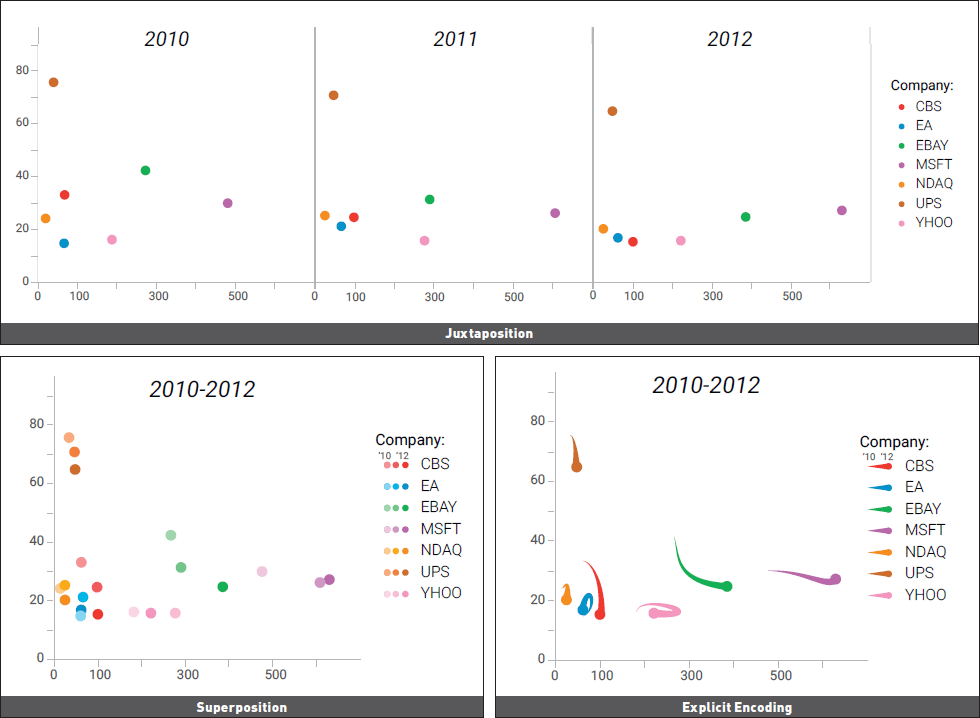
\includegraphics[width=\textwidth]{explicit_encoding}
  \caption{Juxtaposition, Superposition and Explicit Encoding. Image taken from the work of~\cite{Szafir2018}.}
  \label{fig:explicit-endoding-szafir}
\end{figure}

\begin{figure}[H]
  \centering
  \begin{subfigure}[t]{0.75\textwidth}
    \centering
    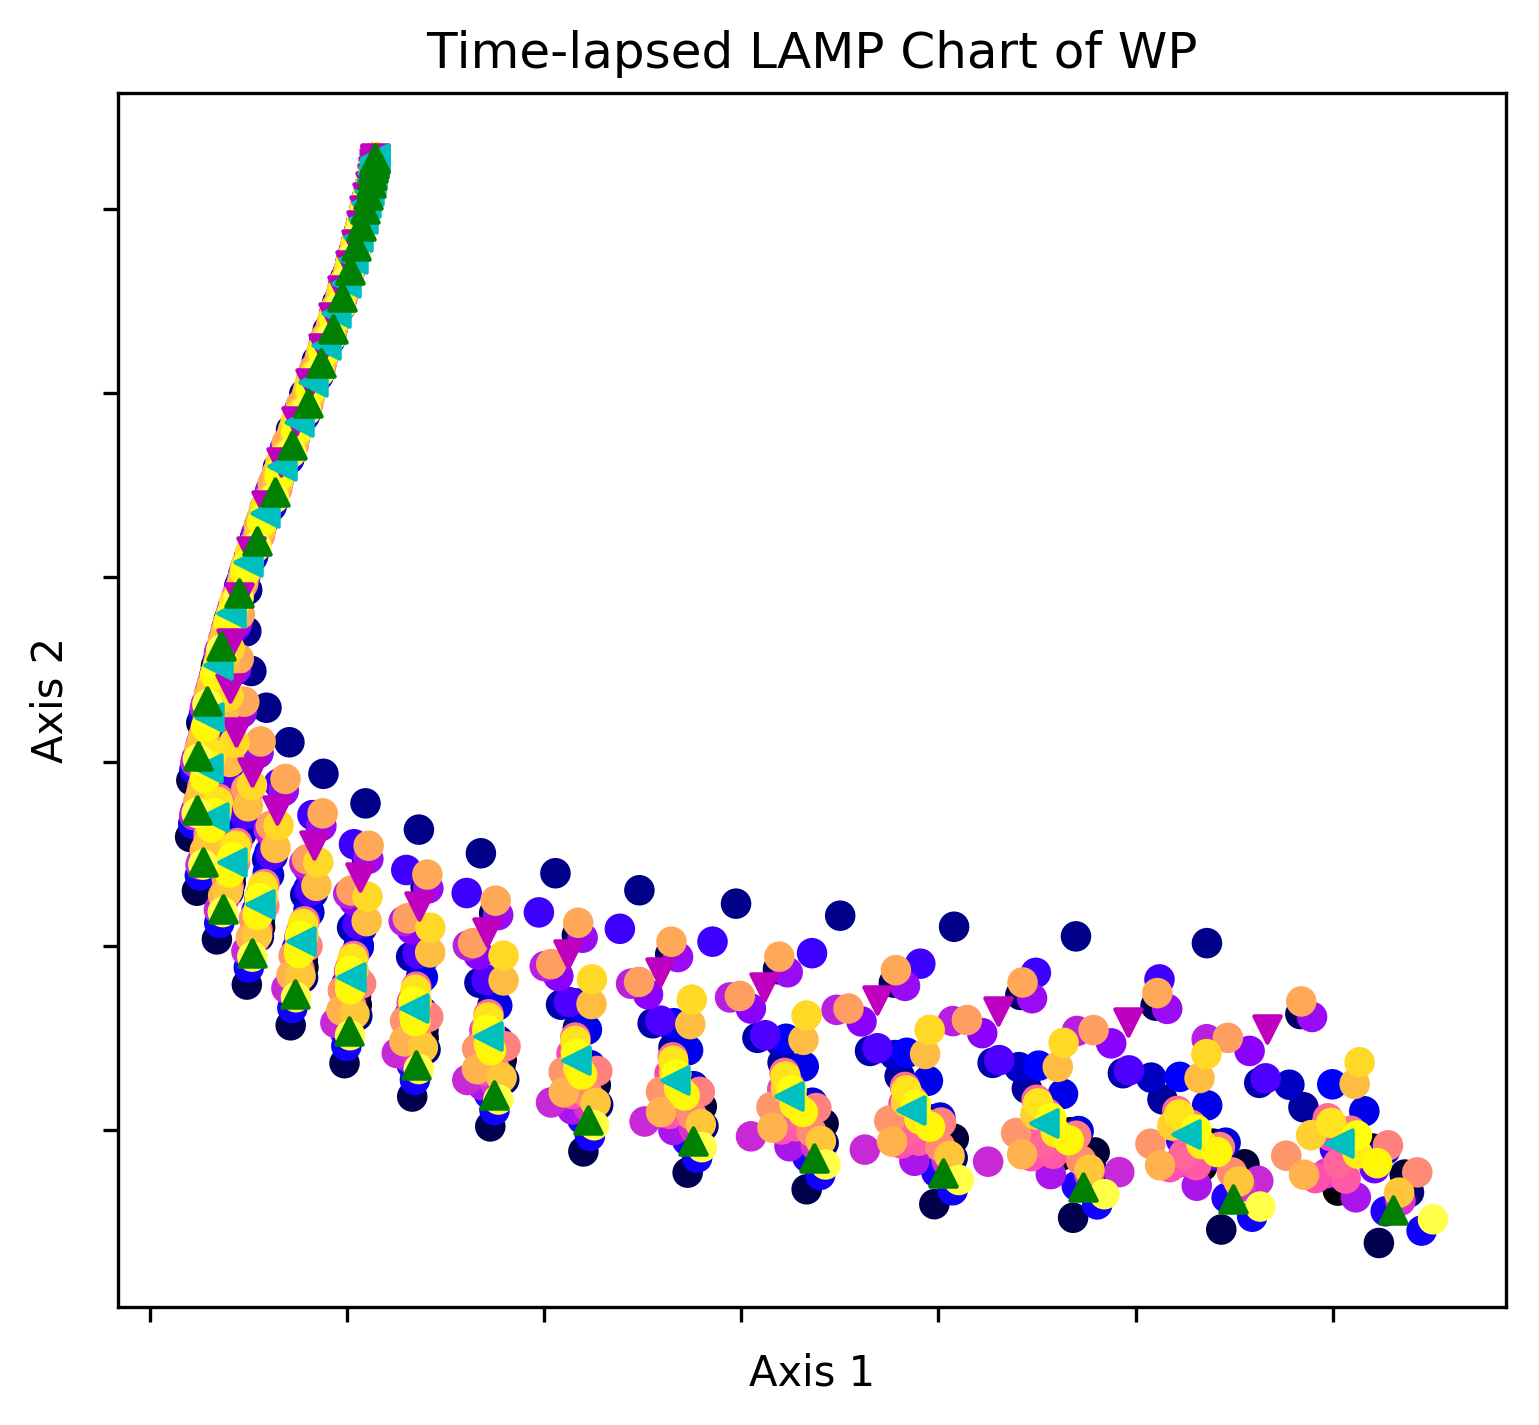
\includegraphics[width=\columnwidth]{WP-tllamp}
    \caption{Superposition of times in the Time-lapsed LAMP chart.}
    \label{fig:superposition-tllamp-inc}
  \end{subfigure}
  ~
  \begin{subfigure}[t]{0.75\textwidth}
    \centering
    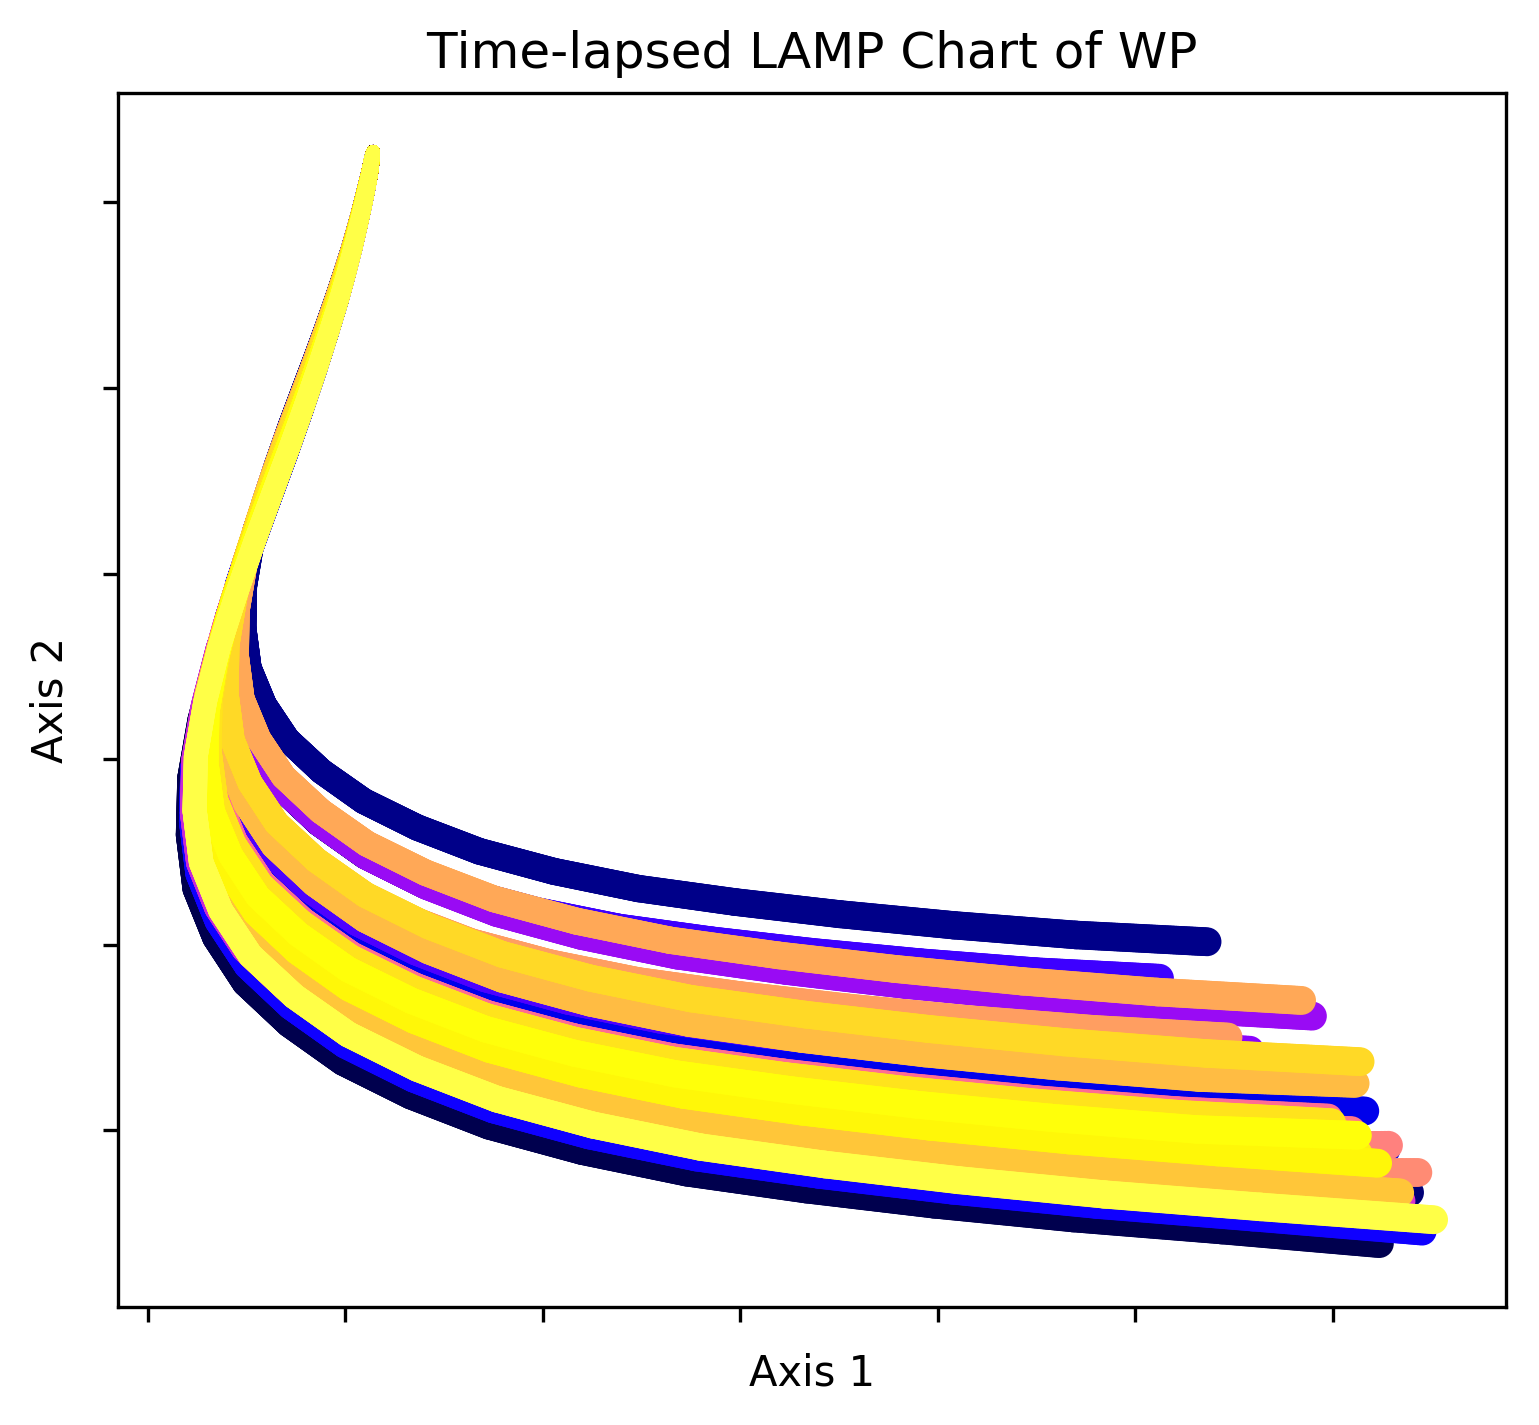
\includegraphics[width=\columnwidth]{WP-tllamp-linear-inc-glyph}
    \caption{Explicit encoding of time in the Time-lapsed LAMP chart. Starting times encoded with smaller glyphs.}
    \label{fig:ee-tllamp-inc}
  \end{subfigure}
  \caption{Comparison between different time encodings on the Time-lapsed LAMP chart of $W_p$. Superposition~(\ref{fig:superposition-tllamp-inc}) and Explicit Encoding~(\ref{fig:ee-tllamp-inc}) from small to large glyphs.}
  \label{fig:explicit-encoding-tllamp-inc}
\end{figure}

%%% Local Variables:
%%% mode: latex
%%% TeX-master: thesis.tex
%%% End:
